\documentclass[tikz, border=20pt]{standalone}
\usepackage{amsmath, amssymb}
\usetikzlibrary{positioning, arrows.meta, fit, backgrounds}

\begin{document}
	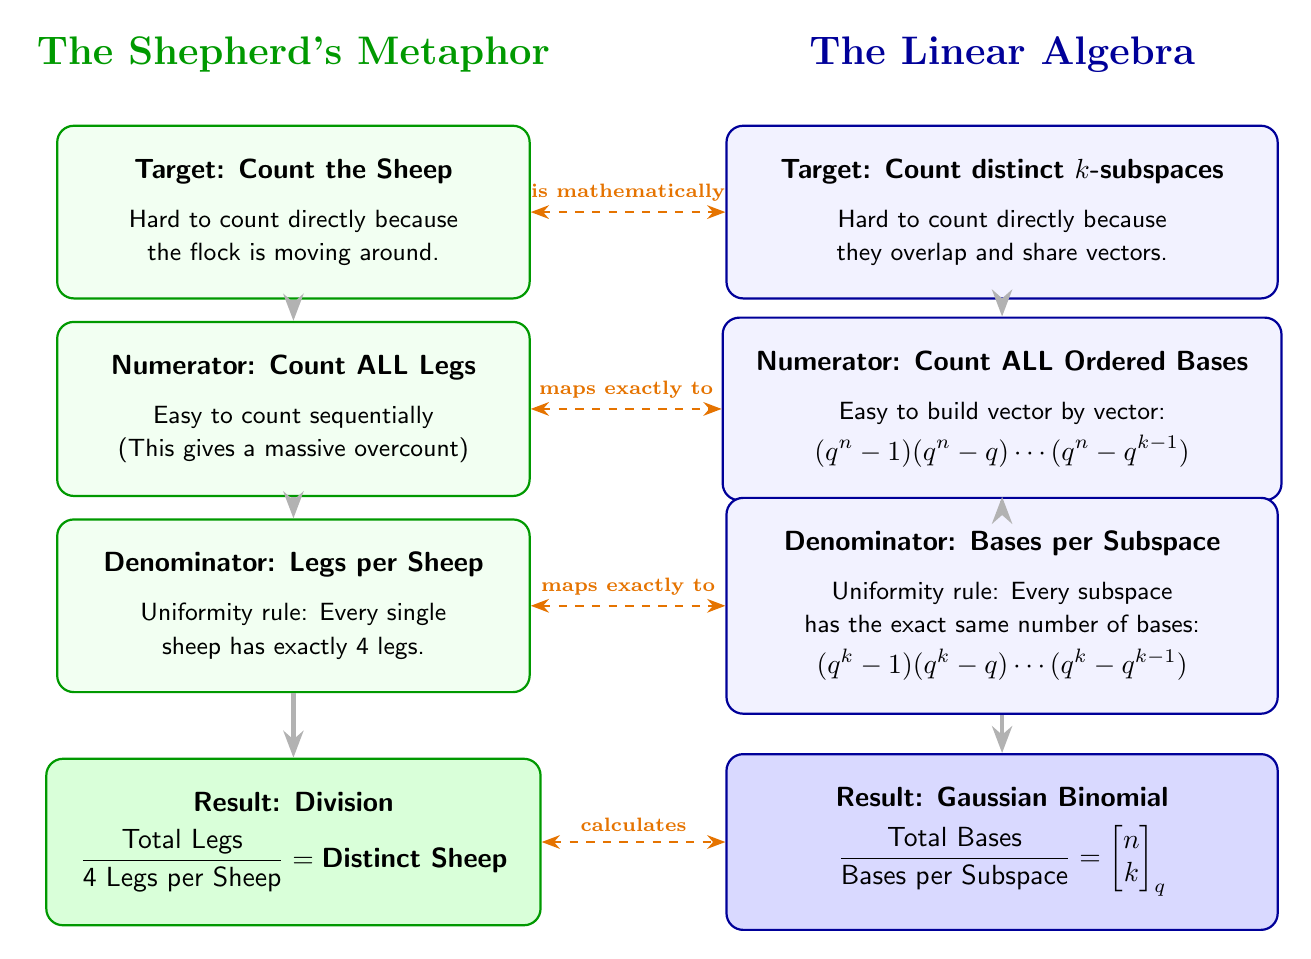
\begin{tikzpicture}[
		font=\sffamily,
		% Box styles for the two columns
		box/.style={draw=black!70, thick, rounded corners=6pt, fill=white, align=center, inner sep=12pt},
		metaphorBox/.style={box, fill=green!5, draw=green!60!black},
		mathBox/.style={box, fill=blue!5, draw=blue!60!black},
		% Arrow styles
		flowArrow/.style={->, >=Stealth, line width=1.5pt, color=gray!60},
		mapArrow/.style={<->, >=Stealth, dashed, thick, color=orange!90!black}
		]
		
		% =========================================================
		% LEFT COLUMN: THE SHEEP METAPHOR
		% =========================================================
		\node[font=\Large\bfseries, text=green!60!black] (MetaTitle) at (-4.5, 4.5) {The Shepherd's Metaphor};
		
		% Step 1: The Goal
		\node[metaphorBox, minimum width=6cm] (MetaGoal) at (-4.5, 2.5) {
			\textbf{Target: Count the Sheep}\\[2mm]
			\small Hard to count directly because\\
			\small the flock is moving around.
		};
		
		% Step 2: The Numerator
		\node[metaphorBox, minimum width=6cm] (MetaNum) at (-4.5, 0) {
			\textbf{Numerator: Count ALL Legs}\\[2mm]
			\small Easy to count sequentially\\
			\small (This gives a massive overcount)
		};
		
		% Step 3: The Denominator
		\node[metaphorBox, minimum width=6cm] (MetaDen) at (-4.5, -2.5) {
			\textbf{Denominator: Legs per Sheep}\\[2mm]
			\small Uniformity rule: Every single\\
			\small sheep has exactly 4 legs.
		};
		
		% Step 4: The Result
		\node[metaphorBox, minimum width=6cm, fill=green!15] (MetaRes) at (-4.5, -5.5) {
			\textbf{Result: Division}\\[2mm]
			$\displaystyle \frac{\text{Total Legs}}{\text{4 Legs per Sheep}} = \textbf{Distinct Sheep}$
		};
		
		% Vertical Flow Arrows (Metaphor)
		\draw[flowArrow] (MetaGoal) -- (MetaNum);
		\draw[flowArrow] (MetaNum) -- (MetaDen);
		\draw[flowArrow] (MetaDen) -- (MetaRes);
		
		
		% =========================================================
		% RIGHT COLUMN: THE MATHEMATICS
		% =========================================================
		\node[font=\Large\bfseries, text=blue!60!black] (MathTitle) at (4.5, 4.5) {The Linear Algebra};
		
		% Step 1: The Goal
		\node[mathBox, minimum width=7cm] (MathGoal) at (4.5, 2.5) {
			\textbf{Target: Count distinct $k$-subspaces}\\[2mm]
			\small Hard to count directly because\\
			\small they overlap and share vectors.
		};
		
		% Step 2: The Numerator
		\node[mathBox, minimum width=7cm] (MathNum) at (4.5, 0) {
			\textbf{Numerator: Count ALL Ordered Bases}\\[2mm]
			\small Easy to build vector by vector:\\[1mm]
			$\displaystyle (q^n-1)(q^n-q)\cdots(q^n-q^{k-1})$
		};
		
		% Step 3: The Denominator
		\node[mathBox, minimum width=7cm] (MathDen) at (4.5, -2.5) {
			\textbf{Denominator: Bases per Subspace}\\[2mm]
			\small Uniformity rule: Every subspace\\
			\small has the exact same number of bases:\\[1mm]
			$\displaystyle (q^k-1)(q^k-q)\cdots(q^k-q^{k-1})$
		};
		
		% Step 4: The Result
		\node[mathBox, minimum width=7cm, fill=blue!15] (MathRes) at (4.5, -5.5) {
			\textbf{Result: Gaussian Binomial}\\[2mm]
			$\displaystyle \frac{\text{Total Bases}}{\text{Bases per Subspace}} = \begin{bmatrix} n \\ k \end{bmatrix}_q$
		};
		
		% Vertical Flow Arrows (Math)
		\draw[flowArrow] (MathGoal) -- (MathNum);
		\draw[flowArrow] (MathNum) -- (MathDen);
		\draw[flowArrow] (MathDen) -- (MathRes);
		
		
		% =========================================================
		% HORIZONTAL MAPPING ARROWS
		% =========================================================
		\draw[mapArrow] (MetaGoal.east) -- (MathGoal.west) node[midway, above, font=\scriptsize\bfseries] {is mathematically};
		\draw[mapArrow] (MetaNum.east) -- (MathNum.west) node[midway, above, font=\scriptsize\bfseries] {maps exactly to};
		\draw[mapArrow] (MetaDen.east) -- (MathDen.west) node[midway, above, font=\scriptsize\bfseries] {maps exactly to};
		\draw[mapArrow] (MetaRes.east) -- (MathRes.west) node[midway, above, font=\scriptsize\bfseries] {calculates};
		
	\end{tikzpicture}
\end{document}